\documentclass[utf8, a4paper]{beamer}

\usepackage[T1]{fontenc}
\usepackage[english]{babel}

\usepackage{amsmath, amsfonts, graphicx}
\usepackage{bibunits, tikz}
\usepackage{animate}

\usetheme{progressbar}

\setbeamersize
  {text margin left=1em, text margin right=1em}

\title
  [Resolution transfer in cancer classification]
  {Resolution transfer in cancer classification based on amplification patterns}

\author
  [Prem Raj Adhikari]
  {\underline{Prem Raj Adhikari}$^{1,2}$\quad Jaakko Hollm\'en$^{1}$}

\date
  {September, 2015}

\institute
{ 
%Helsinki Institute for Information Technology HIIT and \\
$^{1}$ Department Computer Science, Aalto University\\
% PO Box 15400, FI-00076 Aalto, Espoo, Finland\\ 
$^{2}$ Department of Physiology, University of Turku\\
% Kiinamyllynkatu 10, FI-20520 Turku, Finland
}

\begin{document}

\maketitle

% \begin{frame}{Overview}
% 
%   \tableofcontents
% 
% \end{frame}

\section
  {Introduction}


  
  %%%%%%%%%%%%%%%%%%%%%%%%%%%%%%%%%%%%%%%%%%%%%%%%%%%%%%%%%%%%%%%%%%%%%%%%%%%%%%%%%%%%%%%%
\begin{frame} {Elephant and the blind men} 

\vspace{-0.9cm}

\begin{figure}
\centering
  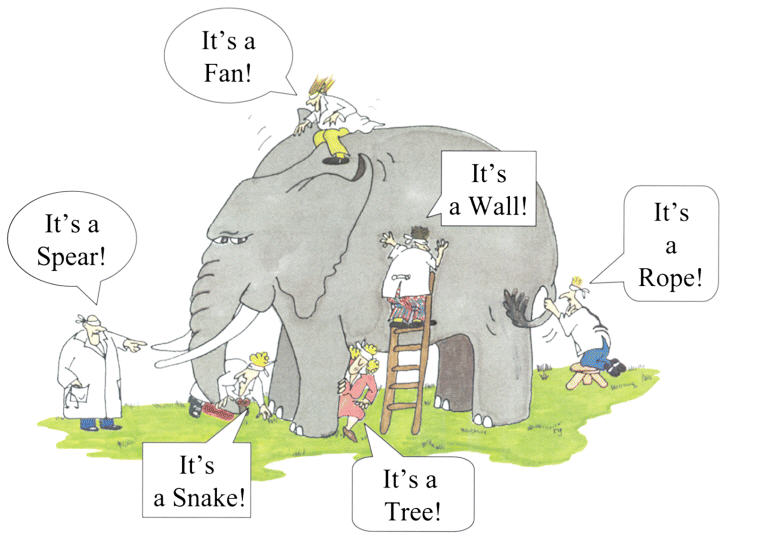
\includegraphics[trim={0cm 0.5cm 0cm 0cm},clip, width=0.77\textwidth]{images/elephant}
\end{figure}

\end{frame}
%%%%%%%%%%%%%%%%%%%%%%%%%%%%%%%%%%%%%%%%%%%%%%%%%%%%%%%%%%%%%%%%%%%%%%%%%%%%%%%%%%%%%%%%
\begin{frame} {In Biology} 

\vspace{-0.9cm}

\begin{figure}
\centering
  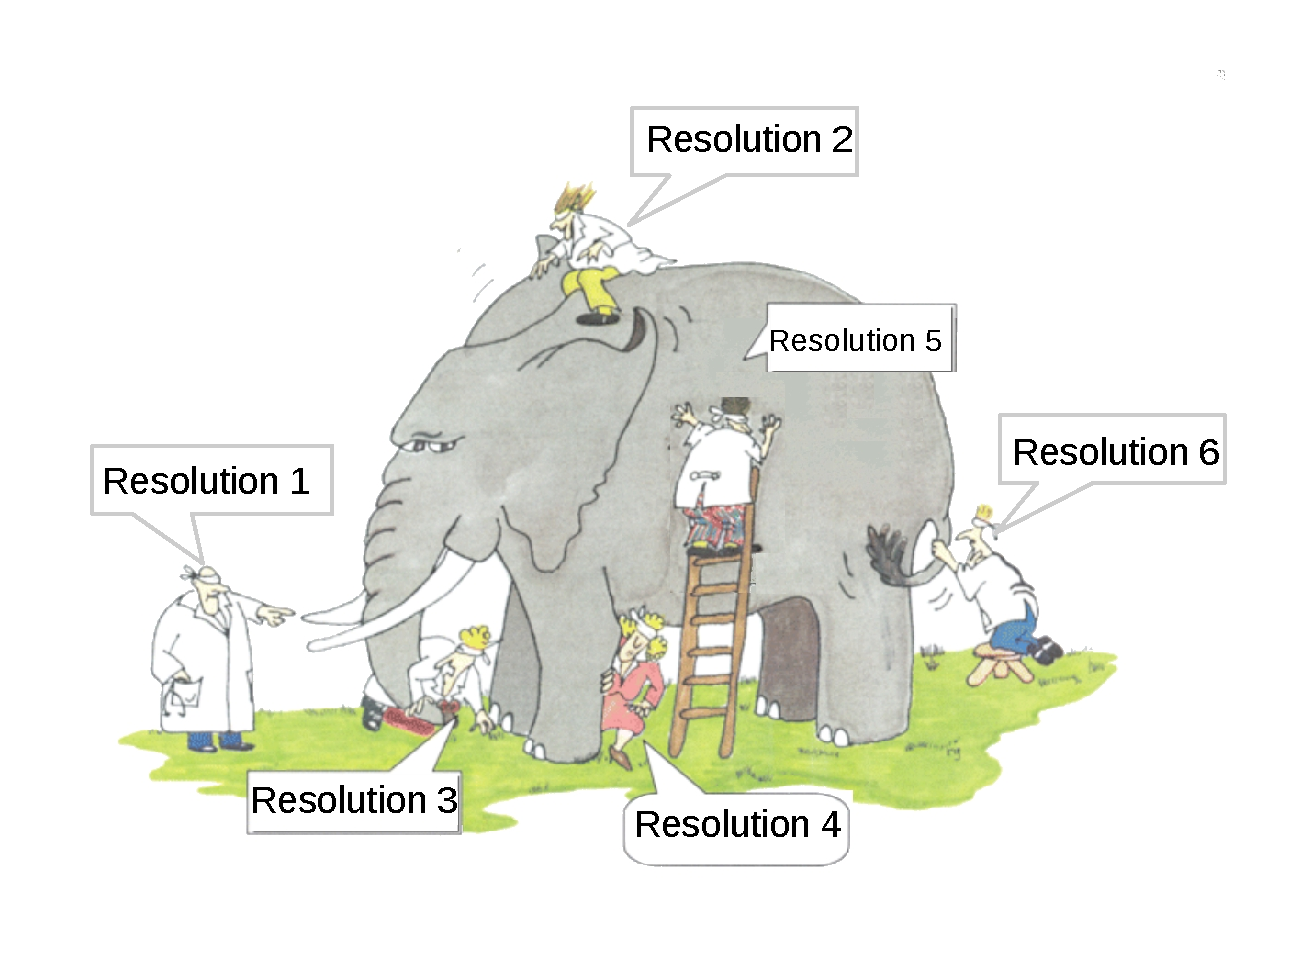
\includegraphics[trim={1cm 1.7cm 1cm 1.7cm},clip, width=0.75\textwidth]{images/elebio_n1}
\end{figure}

\vspace{-1mm}

\tiny Adapted from Y. Moreau, University of Leuven, Belgium

\end{frame}

%%%%%%%%%%%%%%%%%%%%%%%%%%%%%%%%%%%%%%%%%%%%%%%%%%%%%%%%%%%%%%%%%%%%%%%%%%%%%%%%%%%%%%%%
\begin{frame} {Labelled Data} 

\vspace{-0.9cm}

\begin{figure}
\centering
  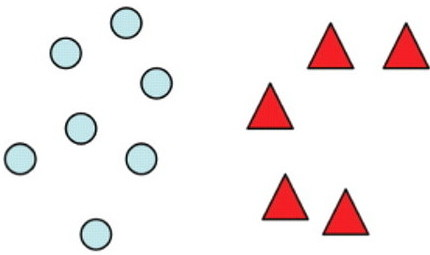
\includegraphics[trim={0cm 0cm 0cm 0cm},clip, width=0.75\textwidth]{images/topleft}
\end{figure}
\tiny{Adapted from Anuj R. Shah, et. al.,  Bioinformatics (2008) }

\end{frame}
%%%%%%%%%%%%%%%%%%%%%%%%%%%%%%%%%%%%%%%%%%%%%%%%%%%%%%%%%%%%%%%%%%%%%%%%%%%%%%%%%%%%%%%%
\begin{frame} {Supervised Learning} 

\vspace{-0.9cm}

\begin{figure}
\centering
  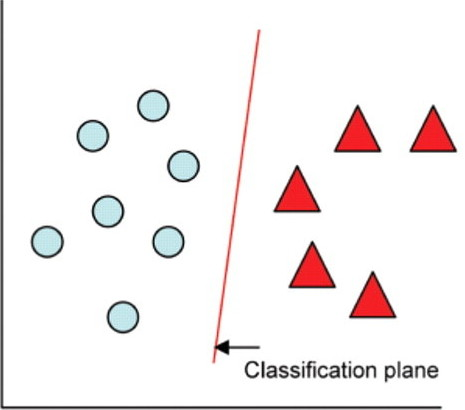
\includegraphics[trim={0cm 0cm 0cm 0cm},clip, width=0.6\textwidth]{images/bottomleft}
\end{figure}

\vspace{0cm}

\tiny{Adapted from Anuj R. Shah, et. al.,  Bioinformatics (2008) }

\end{frame}

%%%%%%%%%%%%%%%%%%%%%%%%%%%%%%%%%%%%%%%%%%%%%%%%%%%%%%%%%%%%%%%%%%%%%%%%%%%%%%%%%%%%%%%%
\begin{frame} {Supervised Learning} 

\vspace{-0.9cm}

\begin{figure}
\centering
  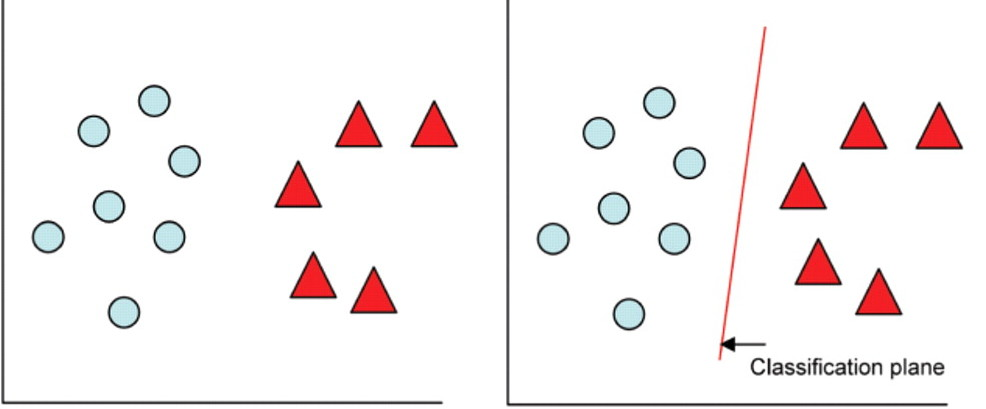
\includegraphics[trim={0cm 0cm 0cm 0cm},clip, width=0.75\textwidth]{images/supervised}
\end{figure}

%\vspace{-0.5cm}

\tiny{Adapted from Anuj R. Shah, et. al.,  Bioinformatics (2008) }

\end{frame}
%%%%%%%%%%%%%%%%%%%%%%%%%%%%%%%%%%%%%%%%%%%%%%%%%%%%%%%%%%%%%%%%%%%%%%%%%%%%%%%%%%%%%%%%
\begin{frame} {Unsupervised Learning} 

\vspace{-0.9cm}

% \begin{figure}
\begin{center}

\animategraphics[scale=0.35, loop,controls]{12}{images/image-}{0}{12}

 
\end{center}

%   \includegraphics[trim={0cm 0cm 0cm 0cm},clip, width=0.75\textwidth]{images/image.gif}
% \end{figure}
%\includemovie{1cm}{1cm}{images/image.gif}

%\vspace{-0.5cm}

\tiny{Adapted from trendsofcode.net }

\end{frame}

%%%%%%%%%%%%%%%%%%%%%%%%%%%%%%%%%%%%%%%%%%%%%%%%%%%%%%%%%%%%%%%%%%%%%%%%%%%%%%%%%%%%%%%%
\begin{frame} {Labelled and Unlabelled Data} 

\vspace{-0.5cm}

\begin{figure}
\centering
  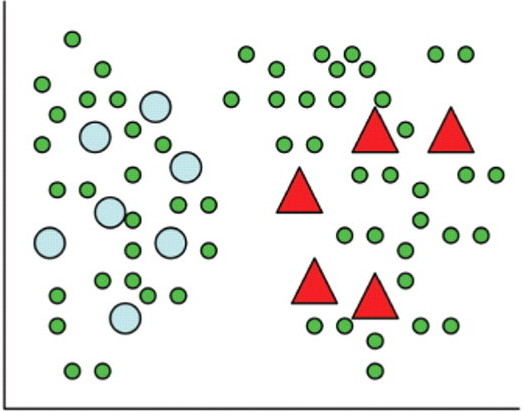
\includegraphics[trim={0cm 0cm 0cm 0cm},clip, width=0.67\textwidth]{images/topright}
\end{figure}

\vspace{-0.3cm}

\tiny{Adapted from Anuj R. Shah, et. al.,  Bioinformatics (2008) }

\end{frame}

%%%%%%%%%%%%%%%%%%%%%%%%%%%%%%%%%%%%%%%%%%%%%%%%%%%%%%%%%%%%%%%%%%%%%%%%%%%%%%%%%%%%%%%%
\begin{frame} {Semisupervised Learning} 

\vspace{-0.9cm}

\begin{figure}
\centering
  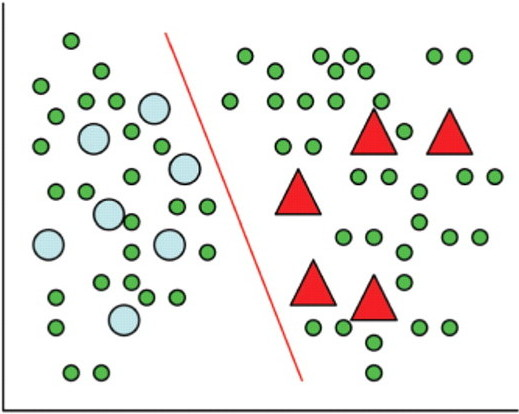
\includegraphics[trim={0cm 0cm 0cm 0cm},clip, width=0.7\textwidth]{images/bottomright}
\end{figure}
\tiny{Adapted from Anuj R. Shah, et. al.,  Bioinformatics (2008) }

\end{frame}

%%%%%%%%%%%%%%%%%%%%%%%%%%%%%%%%%%%%%%%%%%%%%%%%%%%%%%%%%%%%%%%%%%%%%%%%%%%%%%%%%%%%%%%%
\begin{frame} {Semisupervised classification Paradigm} 

\vspace{-0.9cm}

\begin{figure}
\centering
  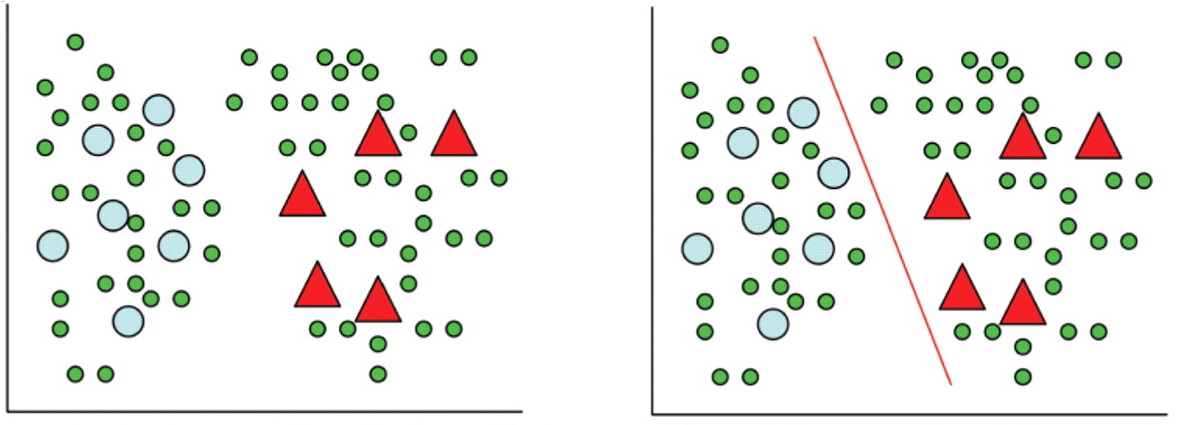
\includegraphics[trim={0cm 0cm 0cm 0cm},clip, width=0.9\textwidth]{images/sermisupervised}
\end{figure}
\tiny{Adapted from Anuj R. Shah, et. al.,  Bioinformatics (2008) }

\end{frame}

%%%%%%%%%%%%%%%%%%%%%%%%%%%%%%%%%%%%%%%%%%%%%%%%%%%%%%%%%%%%%%%%%%%%%%%%%%%%%%%%%%%%%%%%
\begin{frame} {Overall classification Paradigm} 

\vspace{-0.9cm}

\begin{figure}
\centering
  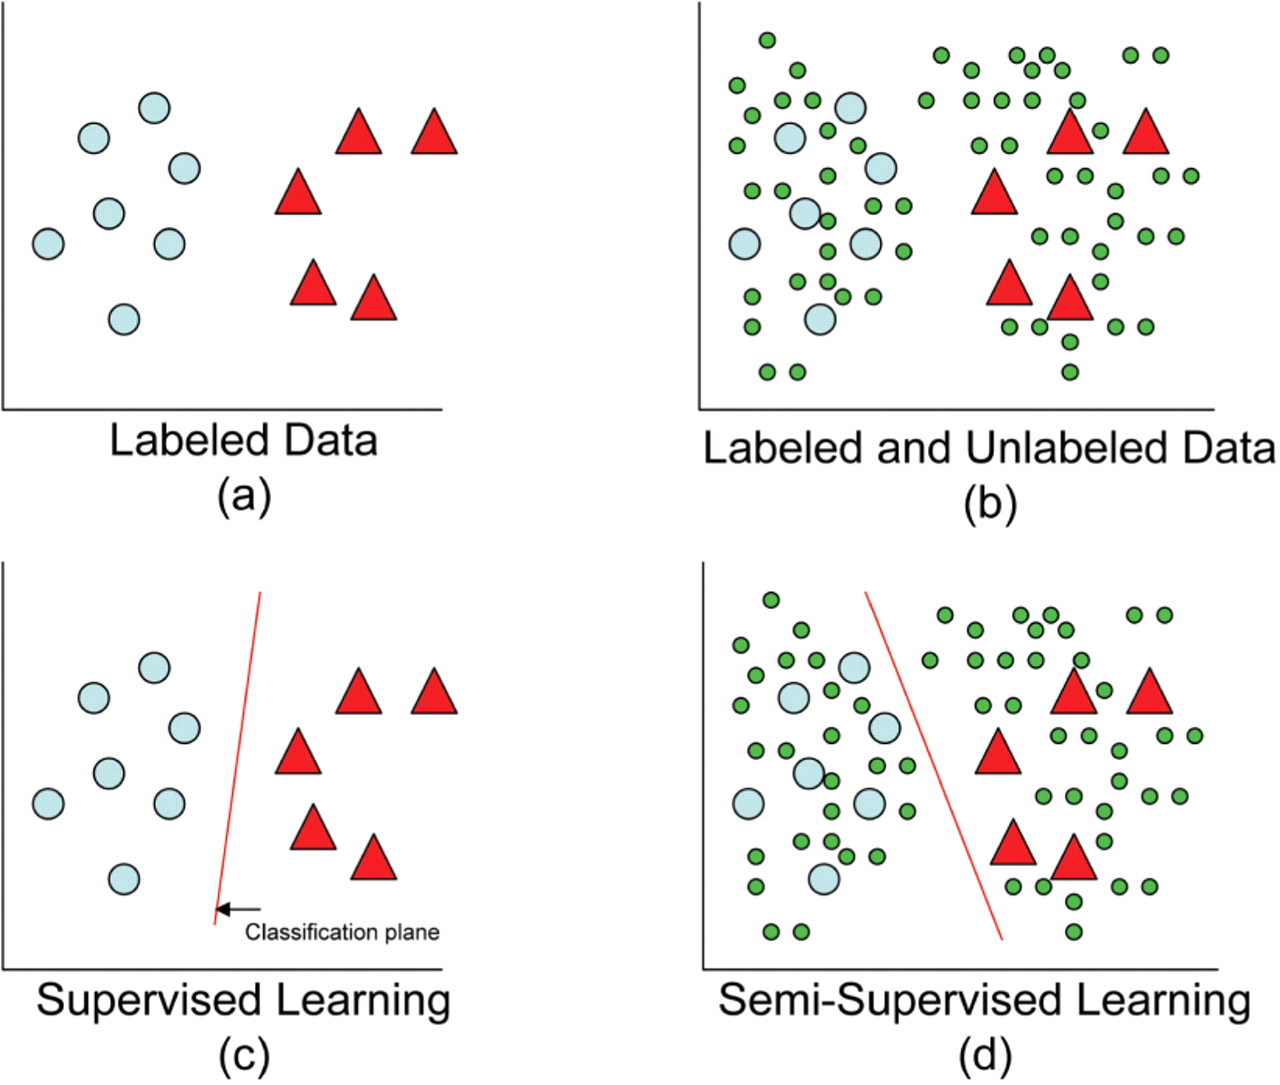
\includegraphics[trim={0cm 0cm 0cm 0cm},clip, width=0.65\textwidth]{images/all}
\end{figure}
\vspace{-0.7cm}
\tiny{Adapted from Anuj R. Shah, et. al.,  Bioinformatics (2008) }
\end{frame}




%%%%%%%%%%%%%%%%%%%%%%%%%%%%%%%%%%%%%%%%%%%%%%%%%%%%%%%%%%%%%%%%%%%%%%%%%%%%%%%%%%%%%%%%

\begin{frame}
  {Challenge: Labelled and Unlabelled Datasets but Different Resolutions }
  \begin{figure}
\centering
  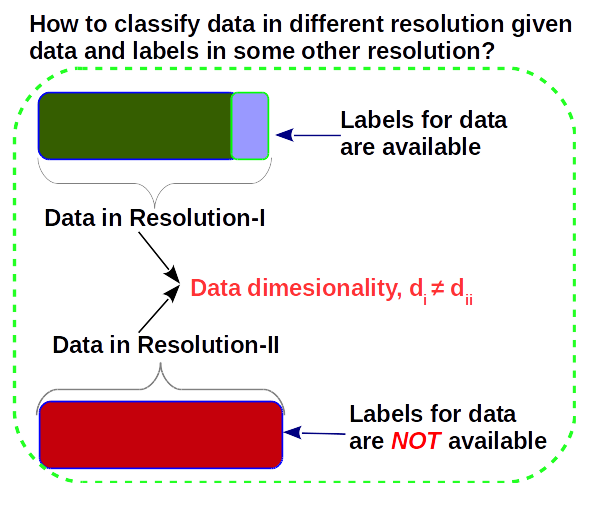
\includegraphics[trim={0cm 0cm 0cm 0cm},clip, width=0.65\textwidth]{images/multires_challenge}
\end{figure}
  
\end{frame}

%%%%%%%%%%%%%%%%%%%%%%%%%%%%%%%%%%%%%%%%%%%%%%%%%%%%%%%%%%%%%%%%%%%%%%%%%%%%%%%%%%%%%%%%

\begin{frame}
  {Solution: Probabilistic Modelling + Transformation}
  
  \vspace{-1cm}
  \begin{figure}
\centering
  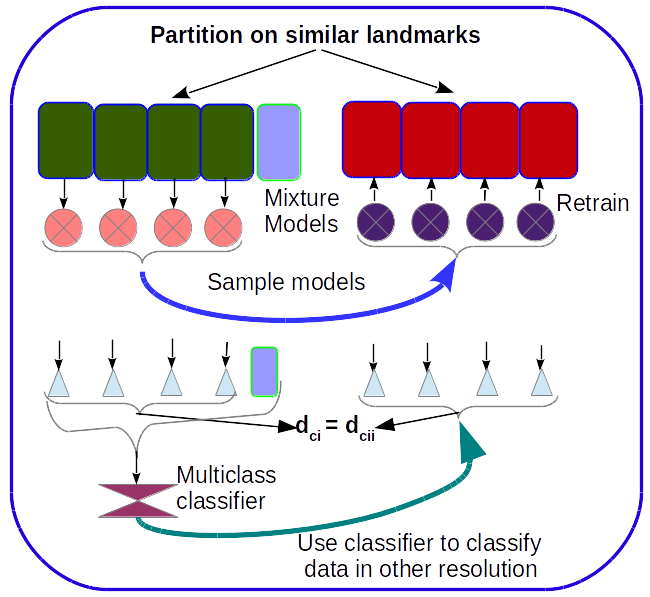
\includegraphics[trim={0cm 0cm 0cm 0cm},clip, width=0.65\textwidth]{images/multires_solution}
\end{figure}
  
\end{frame}

%%%%%%%%%%%%%%%%%%%%%%%%%%%%%%%%%%%%%%%%%%%%%%%%%%%%%%%%%%%%%%%%%%%%%%%%%%%%%%%%%%%%%%%%

\begin{frame}
  {Applications?}
  
  \vspace{-0.5cm}
  \begin{figure}
\centering
  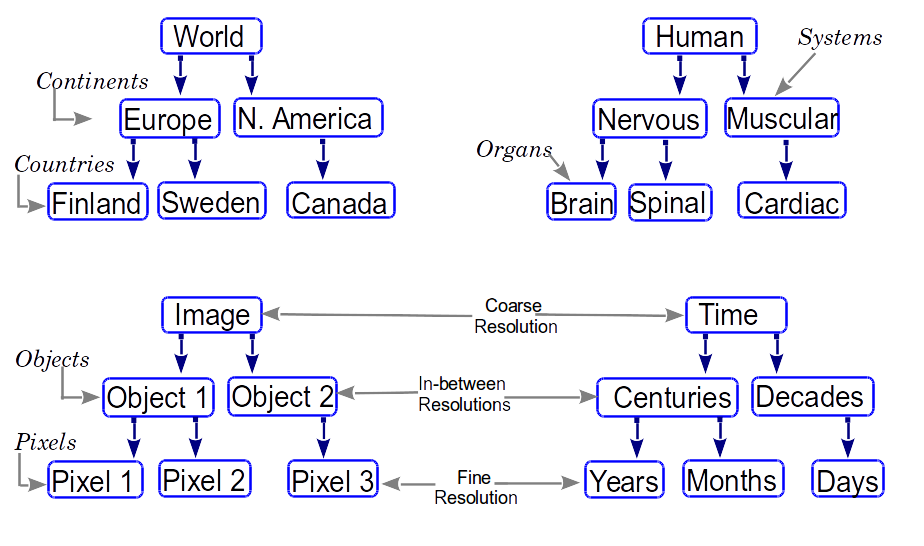
\includegraphics[trim={0cm 0cm 0cm 0cm},clip, width=0.9\textwidth]{images/nonco}
\end{figure}
  
\end{frame}

%%%%%%%%%%%%%%%%%%%%%%%%%%%%%%%%%%%%%%%%%%%%%%%%%%%%%%%%%%%%%%%%%%%%%%%%%%%%%%%%%%%%%%%%


\begin{frame}
  {Multiresolution Chromosomal Aberrations Data}

  \begin{alertblock}
    {Chromosome-wise Mixture Modelling}

    \begin{itemize}
    \itemsep -0.5em 
    \item Divide data into chromosomes! Does not vary with resolution
    \item Train a mixture model for each chromosome in resolution with labels
    \item Append the cluster labels to generate the genome-wide data
    \end{itemize}
  \end{alertblock}
  
  \vspace{-0.1cm}

\begin{figure}
\centering
  \includegraphics[trim={0cm 0cm 0cm 0cm},clip, width=0.98\textwidth]{images/data1}
\end{figure}
  
\end{frame}

%%%%%%%%%%%%%%%%%%%%%%%%%%%%%%%%%%%%%%%%%%%%%%%%%%%%%%%%%%%%%%%%%%%%%%%%%%%%%%%%%%%%%%%%


\section
  {Conclusion}

\begin{bibunit}[plain]
\begin{frame}
  {Transform and retrain the mixture model}
\vspace{-1cm}
\begin{figure}
\centering
  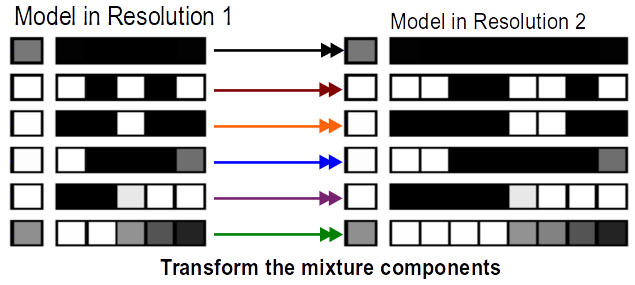
\includegraphics[trim={0cm 0cm 0cm 0cm},clip, width=\textwidth]{images/idasecondpage}
\end{figure}


\end{frame}
\end{bibunit}

%\end{frame}
%\end{bibunit}


%%%%%%%%%%%%%%%%%%%%%%%%%%%%%%%%%%%%%%%%%%%%%%%%%%%%%%%%%%%%%%%%%%%%%%%%%%%%%%%%%%%%%%%%


\begin{frame}
  {Resolution Transfer of Classifier}

  \vspace{0cm}
  \begin{alertblock}
    {Resolution Transfer of Classifier}

    \begin{itemize}
    \itemsep 0em 
    \item Retrain the transformed mixture model and cluster the data 
    \item Append the cluster labels to generate the genome-wide data
    \item Now data in the two resolutions have same dimensionality
    \item Use the trained classifier to classify the genome-wide data
    \end{itemize}
  \end{alertblock}
  
    \begin{alertblock}
    {Chromosomal Aberrations data}

    \begin{itemize}
    \itemsep 0em 
    \item Coarse Resolution 4590 cancer patients (393 dimensionality), 73 different cancer types 
    \item Remove samples with few data points (4104 samples, 34 classes )
    \item Fine resolution data (data dimensionality 850), no class labels (Really!)
   
    \end{itemize}
  \end{alertblock}
  
\end{frame}

%%%%%%%%%%%%%%%%%%%%%%%%%%%%%%%%%%%%%%%%%%%%%%%%%%%%%%%%%%%%%%%%%%%%%%%%%%%%%%%%%%%%%%%%


\begin{frame}
  {Results on Chromosomal Aberrations Dataset}
  \vspace{-1cm}
\begin{figure}
\centering
  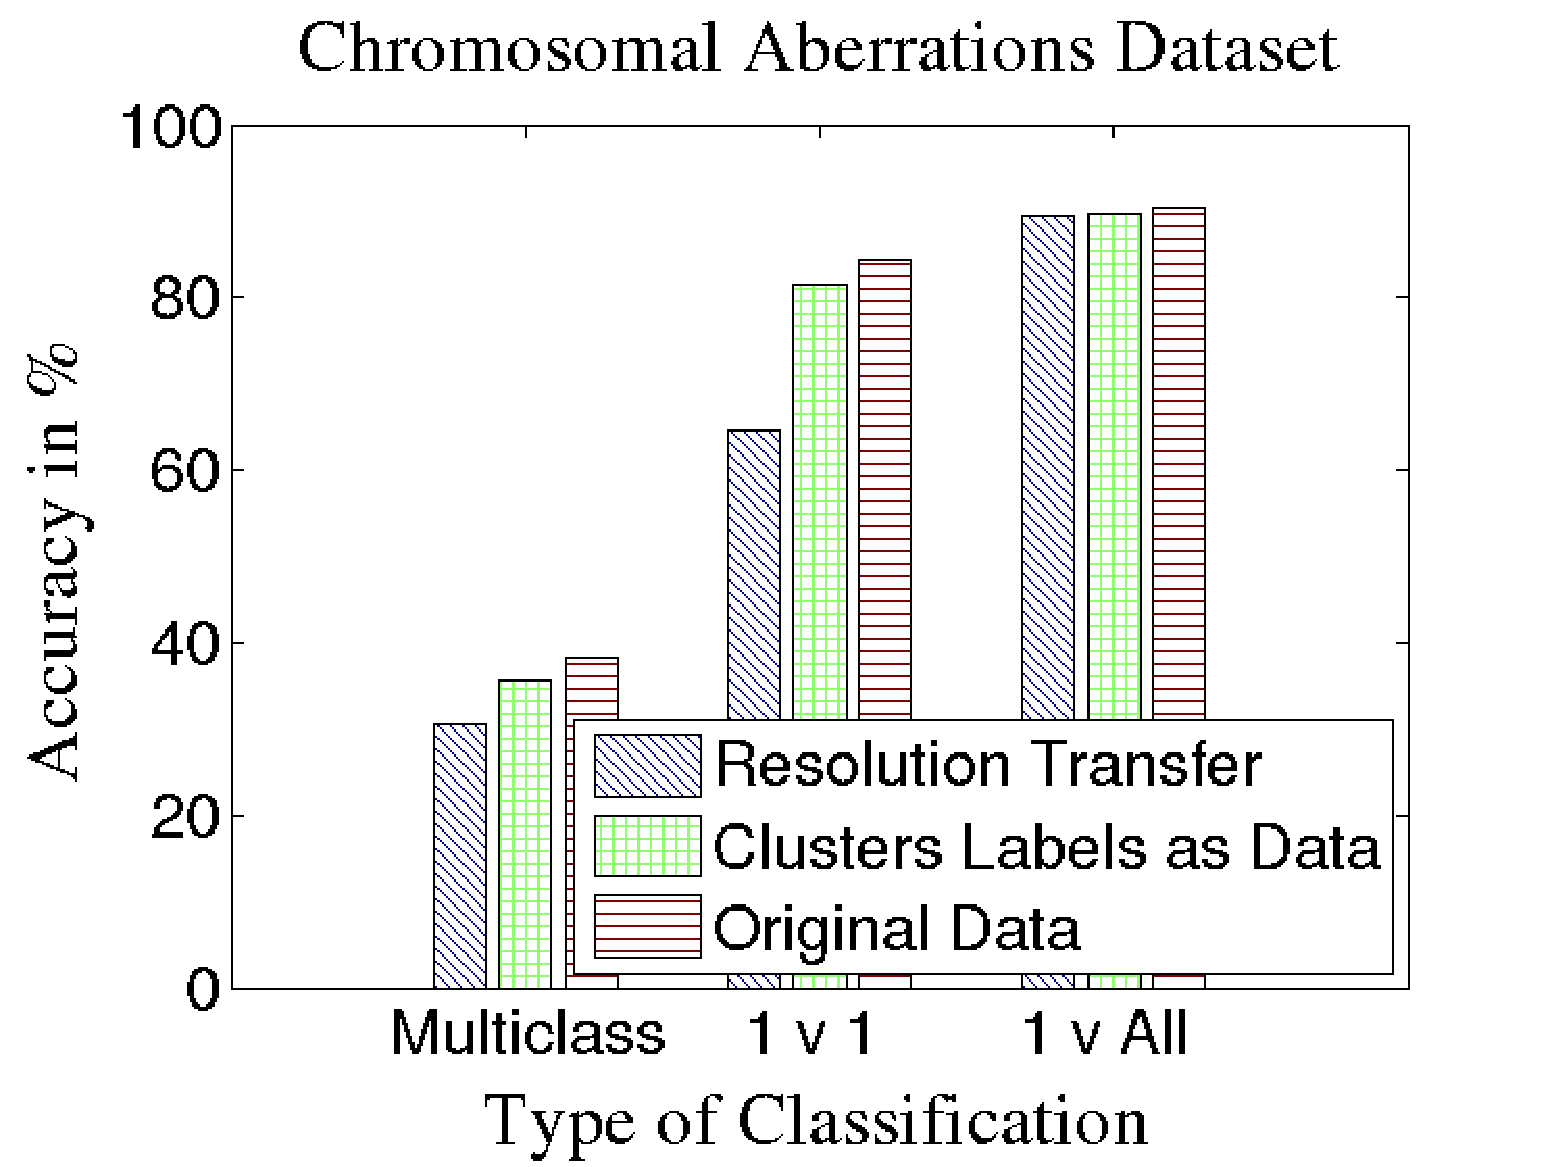
\includegraphics[trim={0cm 0cm 0cm 0cm},clip, width=0.75\textwidth]{images/barlkhood}
\end{figure} 
\end{frame}

%%%%%%%%%%%%%%%%%%%%%%%%%%%%%%%%%%%%%%%%%%%%%%%%%%%%%%%%%%%%%%%%%%%%%%%%%%%%%%%%%%%%%%%%


\begin{frame}
  {Results on Publicly Available Dataset}
  \vspace{-1cm}
\begin{figure}
\centering
  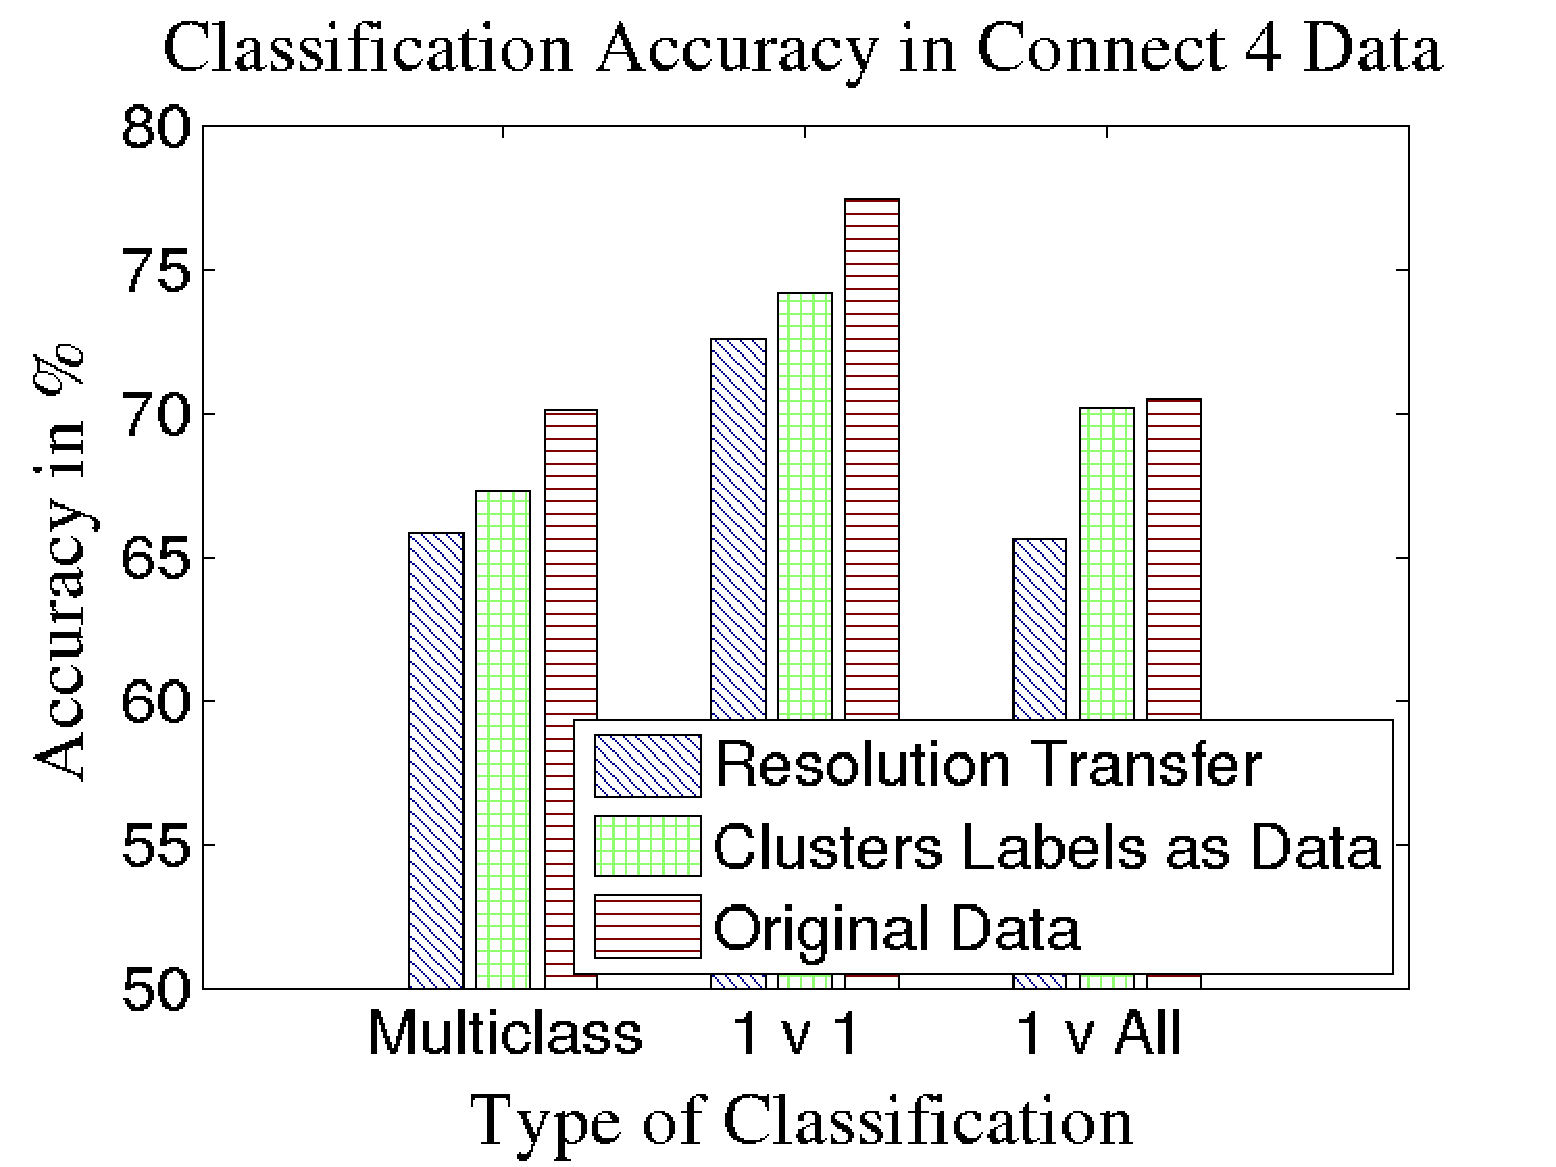
\includegraphics[trim={0cm 0cm 0cm 0cm},clip, width=0.75\textwidth]{images/public}
\end{figure}  
\end{frame}

%%%%%%%%%%%%%%%%%%%%%%%%%%%%%%%%%%%%%%%%%%%%%%%%%%%%%%%%%%%%%%%%%%%%%%%%%%%%%%%%%%%%%%%%


\begin{frame}
  {Summary and Conclusions}
 \begin{itemize}
    \itemsep 1.5em 
    \item Different types of classification algorithms  
    \item Multiple sources of multi-resolution data
    \item Transfer of classifier across different resolutions
    \item Classification of Multiresolution Chromosomal Aberrations dataset and publicly available dataset
    \end{itemize}

\end{frame}



\end{document}


%%% Local Variables:
%%% mode: latex
%%% TeX-master: "demo-slides.tex"
%%% End:
